% -----------------------------------------------
% chktex-file 44
\documentclass[../index.tex]{subfiles}

% -----------------------------------------------

\begin{document}

% -----------------------------------------------
\renewcommand{\sectiontitle}{Let's talk about the web}
\section{\sectiontitle}
% Without getting into much detail, let's get a brief high-level overview of what happens when
% you go on a website in your web browser.

% ---------------------------
\renewcommand{\currenttitle}{\sectiontitle}
\begin{frame}[fragile]{\currenttitle}
% Here's a pretty barebones diagram of a generic client-server architecture.
%
% The client process will send a request to the server, which is running a loop to listen for
% requests.
% When the server receives the request, it'll do some action and then return a response.
% The client will be waiting for the response, and when it gets it, it'll maybe do something
% based on that response.
%
% So you have this loop of client making requests and server returning responses.
%
% Remember that this is a rather generic pattern, so it can be applied to many things.
  \begin{figure}
    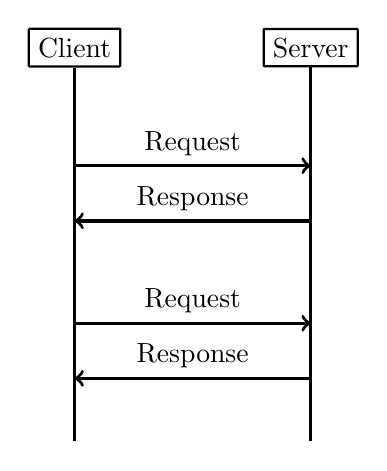
\begin{tikzpicture}[every node/.append style={thick,rounded corners=0.1mm}]
      \node[draw,rectangle] (Client) at (0,0) {Client};
      \node[draw,rectangle] (Server) at (3,0) {Server};

      \draw [very thick] (Client)--++(0,-5);
      \draw [very thick] (Server)--++(0,-5);

      \draw [->,very thick] (0,-1.5)--node [auto] {Request}++(3,0);
      \draw [<-,very thick] (0,-2.2)--node [auto] {Response}++(3,0);

      \draw [->,very thick] (0,-3.5)--node [auto] {Request}++(3,0);
      \draw [<-,very thick] (0,-4.2)--node [auto] {Response}++(3,0);
    \end{tikzpicture}
    \caption{Client-server communication}
  \end{figure}
\end{frame}

% ---------------------------
\begin{frame}[fragile]{\currenttitle}
% In our case, we're talking about the web, so let's make this diagram a little more specific.
%
% The modern web is dominated by a protocol known as HTTP. You've probably heard these letters
% strung together before.
% It stands for Hyper-Text Transfer Protocol.
% This is the protocol the client and server use to send and receive requests and responses.
%
% So, the client, in our case, the web browser or some other web client, will send what we'll
% call an HTTP request.
% The server receives, it does something, and return a response.
%
% The technical specifics of HTTP or any other network protocol is way out of the scope of this
% workshop, so we'll just leave it at that.
  \begin{figure}
    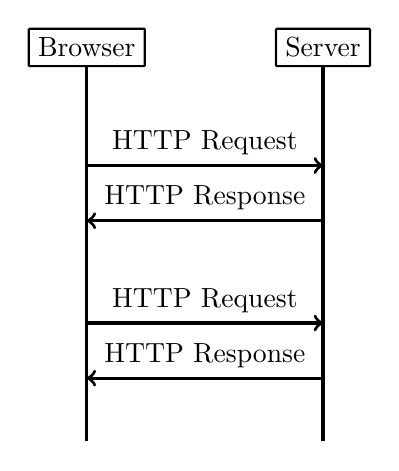
\begin{tikzpicture}[every node/.append style={thick,rounded corners=0.1mm}]
      \node[draw,rectangle] (Client) at (0,0) {Browser};
      \node[draw,rectangle] (Server) at (3,0) {Server};

      \draw [very thick] (Client)--++(0,-5);
      \draw [very thick] (Server)--++(0,-5);

      \draw [->,very thick] (0,-1.5)--node [auto] {HTTP Request} ++(3,0);
      \draw [<-,very thick] (0,-2.2)--node [auto] {HTTP Response}++(3,0);

      \draw [->,very thick] (0,-3.5)--node [auto] {HTTP Request} ++(3,0);
      \draw [<-,very thick] (0,-4.2)--node [auto] {HTTP Response}++(3,0);
    \end{tikzpicture}
    \caption{Client-server HTTP communication}
  \end{figure}
\end{frame}

% ---------------------------
\renewcommand{\currenttitle}{HTTP request methods}
\begin{frame}{\currenttitle}
% What you do need to know is that there are different types of HTTP requests.
% We call these methods.
%
% The most common ones are outlined in this table: GET, POST, PUT, and DELETE.
  \begin{table}
    \begin{tabular}{| l | l | p{0.65\textwidth} |} \hline
      Method  & Payload & Description \\ \hline
      GET     & No      & Request some resource. \\
      POST    & Yes     & Create some resource, usually resulting in a state change. \\
      PUT     & Yes     & Update some resource. \\
      DELETE  & No      & Delete some resource. \\ \hline
    \end{tabular}
    \caption{HTTP request methods}
  \end{table}
\end{frame}

% ---------------------------
\begin{frame}[fragile]{\currenttitle}
% The GET request is pretty much what it sounds like: a request to get the value
% of something.
% We'll use the term 'resource' to generically refer to 'something'.
  W

\end{frame}

% ---------------------------
\begin{frame}[fragile]{\currenttitle}
% The POST request is typically made when you create something in the server.
% Let's say your server maintains a database of users.
% A POST request cause the backend to create a user.
% POST requests typically have a payload, or body.
\end{frame}


% -----------------------------------------------

\end{document}
